% Options for packages loaded elsewhere
\PassOptionsToPackage{unicode}{hyperref}
\PassOptionsToPackage{hyphens}{url}
\documentclass[
]{article}
\usepackage{xcolor}
\usepackage[margin=1in]{geometry}
\usepackage{amsmath,amssymb}
\setcounter{secnumdepth}{5}
\usepackage{iftex}
\ifPDFTeX
  \usepackage[T1]{fontenc}
  \usepackage[utf8]{inputenc}
  \usepackage{textcomp} % provide euro and other symbols
\else % if luatex or xetex
  \usepackage{unicode-math} % this also loads fontspec
  \defaultfontfeatures{Scale=MatchLowercase}
  \defaultfontfeatures[\rmfamily]{Ligatures=TeX,Scale=1}
\fi
\usepackage{lmodern}
\ifPDFTeX\else
  % xetex/luatex font selection
\fi
% Use upquote if available, for straight quotes in verbatim environments
\IfFileExists{upquote.sty}{\usepackage{upquote}}{}
\IfFileExists{microtype.sty}{% use microtype if available
  \usepackage[]{microtype}
  \UseMicrotypeSet[protrusion]{basicmath} % disable protrusion for tt fonts
}{}
\makeatletter
\@ifundefined{KOMAClassName}{% if non-KOMA class
  \IfFileExists{parskip.sty}{%
    \usepackage{parskip}
  }{% else
    \setlength{\parindent}{0pt}
    \setlength{\parskip}{6pt plus 2pt minus 1pt}}
}{% if KOMA class
  \KOMAoptions{parskip=half}}
\makeatother
\usepackage{color}
\usepackage{fancyvrb}
\newcommand{\VerbBar}{|}
\newcommand{\VERB}{\Verb[commandchars=\\\{\}]}
\DefineVerbatimEnvironment{Highlighting}{Verbatim}{commandchars=\\\{\}}
% Add ',fontsize=\small' for more characters per line
\usepackage{framed}
\definecolor{shadecolor}{RGB}{248,248,248}
\newenvironment{Shaded}{\begin{snugshade}}{\end{snugshade}}
\newcommand{\AlertTok}[1]{\textcolor[rgb]{0.94,0.16,0.16}{#1}}
\newcommand{\AnnotationTok}[1]{\textcolor[rgb]{0.56,0.35,0.01}{\textbf{\textit{#1}}}}
\newcommand{\AttributeTok}[1]{\textcolor[rgb]{0.13,0.29,0.53}{#1}}
\newcommand{\BaseNTok}[1]{\textcolor[rgb]{0.00,0.00,0.81}{#1}}
\newcommand{\BuiltInTok}[1]{#1}
\newcommand{\CharTok}[1]{\textcolor[rgb]{0.31,0.60,0.02}{#1}}
\newcommand{\CommentTok}[1]{\textcolor[rgb]{0.56,0.35,0.01}{\textit{#1}}}
\newcommand{\CommentVarTok}[1]{\textcolor[rgb]{0.56,0.35,0.01}{\textbf{\textit{#1}}}}
\newcommand{\ConstantTok}[1]{\textcolor[rgb]{0.56,0.35,0.01}{#1}}
\newcommand{\ControlFlowTok}[1]{\textcolor[rgb]{0.13,0.29,0.53}{\textbf{#1}}}
\newcommand{\DataTypeTok}[1]{\textcolor[rgb]{0.13,0.29,0.53}{#1}}
\newcommand{\DecValTok}[1]{\textcolor[rgb]{0.00,0.00,0.81}{#1}}
\newcommand{\DocumentationTok}[1]{\textcolor[rgb]{0.56,0.35,0.01}{\textbf{\textit{#1}}}}
\newcommand{\ErrorTok}[1]{\textcolor[rgb]{0.64,0.00,0.00}{\textbf{#1}}}
\newcommand{\ExtensionTok}[1]{#1}
\newcommand{\FloatTok}[1]{\textcolor[rgb]{0.00,0.00,0.81}{#1}}
\newcommand{\FunctionTok}[1]{\textcolor[rgb]{0.13,0.29,0.53}{\textbf{#1}}}
\newcommand{\ImportTok}[1]{#1}
\newcommand{\InformationTok}[1]{\textcolor[rgb]{0.56,0.35,0.01}{\textbf{\textit{#1}}}}
\newcommand{\KeywordTok}[1]{\textcolor[rgb]{0.13,0.29,0.53}{\textbf{#1}}}
\newcommand{\NormalTok}[1]{#1}
\newcommand{\OperatorTok}[1]{\textcolor[rgb]{0.81,0.36,0.00}{\textbf{#1}}}
\newcommand{\OtherTok}[1]{\textcolor[rgb]{0.56,0.35,0.01}{#1}}
\newcommand{\PreprocessorTok}[1]{\textcolor[rgb]{0.56,0.35,0.01}{\textit{#1}}}
\newcommand{\RegionMarkerTok}[1]{#1}
\newcommand{\SpecialCharTok}[1]{\textcolor[rgb]{0.81,0.36,0.00}{\textbf{#1}}}
\newcommand{\SpecialStringTok}[1]{\textcolor[rgb]{0.31,0.60,0.02}{#1}}
\newcommand{\StringTok}[1]{\textcolor[rgb]{0.31,0.60,0.02}{#1}}
\newcommand{\VariableTok}[1]{\textcolor[rgb]{0.00,0.00,0.00}{#1}}
\newcommand{\VerbatimStringTok}[1]{\textcolor[rgb]{0.31,0.60,0.02}{#1}}
\newcommand{\WarningTok}[1]{\textcolor[rgb]{0.56,0.35,0.01}{\textbf{\textit{#1}}}}
\usepackage{longtable,booktabs,array}
\usepackage{calc} % for calculating minipage widths
% Correct order of tables after \paragraph or \subparagraph
\usepackage{etoolbox}
\makeatletter
\patchcmd\longtable{\par}{\if@noskipsec\mbox{}\fi\par}{}{}
\makeatother
% Allow footnotes in longtable head/foot
\IfFileExists{footnotehyper.sty}{\usepackage{footnotehyper}}{\usepackage{footnote}}
\makesavenoteenv{longtable}
\usepackage{graphicx}
\makeatletter
\newsavebox\pandoc@box
\newcommand*\pandocbounded[1]{% scales image to fit in text height/width
  \sbox\pandoc@box{#1}%
  \Gscale@div\@tempa{\textheight}{\dimexpr\ht\pandoc@box+\dp\pandoc@box\relax}%
  \Gscale@div\@tempb{\linewidth}{\wd\pandoc@box}%
  \ifdim\@tempb\p@<\@tempa\p@\let\@tempa\@tempb\fi% select the smaller of both
  \ifdim\@tempa\p@<\p@\scalebox{\@tempa}{\usebox\pandoc@box}%
  \else\usebox{\pandoc@box}%
  \fi%
}
% Set default figure placement to htbp
\def\fps@figure{htbp}
\makeatother
\setlength{\emergencystretch}{3em} % prevent overfull lines
\providecommand{\tightlist}{%
  \setlength{\itemsep}{0pt}\setlength{\parskip}{0pt}}
\usepackage[]{natbib}
\bibliographystyle{plainnat}
\usepackage{bookmark}
\IfFileExists{xurl.sty}{\usepackage{xurl}}{} % add URL line breaks if available
\urlstyle{same}
\hypersetup{
  pdftitle={Lab 08 - University of Edinburgh Art Collection},
  pdfauthor={Tina Huynh},
  hidelinks,
  pdfcreator={LaTeX via pandoc}}

\title{Lab 08 - University of Edinburgh Art Collection}
\author{Tina Huynh}
\date{}

\begin{document}
\maketitle

{
\setcounter{tocdepth}{2}
\tableofcontents
}
The University of Edinburgh Art Collection \emph{``supports the
world-leading research and teaching that happens within the University.
Comprised of an astonishing range of objects and ideas spanning two
millennia and a multitude of artistic forms, the collection reflects not
only the long and rich trajectory of the University, but also major
national and international shifts in art history.''}\footnote{Source:
  \url{https://collections.ed.ac.uk/art/about}}.

\begin{verbatim}
See the sidebar [here](https://collections.ed.ac.uk/art) and note that there are 2970 pieces in the art collection we're collecting data on. Note that more pieces may have been added or some pieces may have been removed between when this lab was written and when you're working on it.
\end{verbatim}

In this lab we'll scrape data on all art pieces in the
\href{https://collections.ed.ac.uk/art/search/*:*/Collection:\%22edinburgh+college+of+art\%7C\%7C\%7CEdinburgh+College+of+Art\%22}{Edinburgh
College of Art collection}.

\section{Learning goals}\label{learning-goals}

\begin{itemize}
\tightlist
\item
  Working with R scripts
\item
  Web scraping from a single page
\item
  Writing functions
\item
  Iteration by mapping functions
\item
  Writing data out
\end{itemize}

\section{Lab prep}\label{lab-prep}

\pandocbounded{
\includegraphics[keepaspectratio]{img/selectorgadget.png}}

\begin{itemize}
\item
  Download and install the SelectorGadget for your browser. Once you do,
  you should now be able to access SelectorGadget by clicking on the
  icon next to the search bar in your Chrome or Firefox browser.

  \begin{itemize}
  \tightlist
  \item
    See
    \href{https://chrome.google.com/webstore/detail/selectorgadget/mhjhnkcfbdhnjickkkdbjoemdmbfginb}{here}
    for Chrome (recommended)
  \item
    See
    \href{https://addons.mozilla.org/en-US/firefox/addon/chropath-for-firefox}{here}
    for Firefox
  \end{itemize}
\item
  Read the following on working with R Markdown documents vs.~R scripts.
\end{itemize}

\subsection{R scripts vs.~R Markdown
documents}\label{r-scripts-vs.-r-markdown-documents}

Today we will be using both R scripts and R Markdown documents:

\begin{itemize}
\item
  \texttt{.R}: R scripts are plain text files containing \textbf{only}
  code and brief comments,

  \begin{itemize}
  \tightlist
  \item
    We'll use R scripts in the web scraping stage and ultimately save
    the scraped data as a csv.
  \end{itemize}
\item
  \texttt{.Rmd}: R Markdown documents are plain text files containing.

  \begin{itemize}
  \tightlist
  \item
    We'll use an R Markdown document in the web analysis stage, where we
    start off by reading in the csv file we wrote out in the scraping
    stage.
  \end{itemize}
\end{itemize}

Here is the organization of your repo, and the corresponding section in
the lab that each file will be used for:

\section{Getting started}\label{getting-started}

Go to the course GitHub organization and locate your homework repo,
clone it in RStudio and open the R Markdown document. Knit the document
to make sure it compiles without errors.

\subsection{Warm up}\label{warm-up}

Let's warm up with some simple exercises. Update the YAML of your R
Markdown file with your information, knit, commit, and push your
changes. Make sure to commit with a meaningful commit message. Then, go
to your repo on GitHub and confirm that your changes are visible in your
Rmd \textbf{and} md files. If anything is missing, commit and push
again.

\subsection{Packages}\label{packages}

We'll use the \textbf{tidyverse} package for much of the data wrangling
and visualisation, the \textbf{robotstxt} package to check if we're
allowed to scrape the data, the \textbf{rvest} package for data
scraping. These packages are already installed for you. You can load
them by running the following in your Console:

\begin{Shaded}
\begin{Highlighting}[]
\FunctionTok{library}\NormalTok{(tidyverse)}
\FunctionTok{library}\NormalTok{(robotstxt)}
\FunctionTok{library}\NormalTok{(rvest)}
\end{Highlighting}
\end{Shaded}

\subsection{Data}\label{data}

This assignment does not come with any prepared datasets. Instead you'll
be scraping the data! But before doing so, let's check that a bot has
permissions to access pages on this domain.

\begin{Shaded}
\begin{Highlighting}[]
\FunctionTok{paths\_allowed}\NormalTok{(}\StringTok{"https://collections.ed.ac.uk/art)"}\NormalTok{)}
\end{Highlighting}
\end{Shaded}

\begin{verbatim}
##  collections.ed.ac.uk
\end{verbatim}

\begin{verbatim}
## [1] TRUE
\end{verbatim}

\section{Exercises}\label{exercises}

\subsection{Scraping a single page}\label{scraping-a-single-page}

\begin{verbatim}
**Tip:** To run the code you can highlight or put your cursor next to the lines of code you want to run and hit Command+Enter.
\end{verbatim}

Work in \texttt{scripts/01-scrape-page-one.R}.

We will start off by scraping data on the first 10 pieces in the
collection from
\href{https://collections.ed.ac.uk/art/search/*:*/Collection:\%22edinburgh+college+of+art\%7C\%7C\%7CEdinburgh+College+of+Art\%22?offset=0}{here}.

First, we define a new object called \texttt{first\_url}, which is the
link above. Then, we read the page at this url with the
\texttt{read\_html()} function from the \textbf{rvest} package. The code
for this is already provided in \texttt{01-scrape-page-one.R}.

\begin{Shaded}
\begin{Highlighting}[]
\CommentTok{\# set url}
\NormalTok{first\_url }\OtherTok{\textless{}{-}} \StringTok{"https://collections.ed.ac.uk/art/search/*:*/Collection:\%22edinburgh+college+of+art\%7C\%7C\%7CEdinburgh+College+of+Art\%22?offset=0"}

\CommentTok{\# read html page}
\NormalTok{page }\OtherTok{\textless{}{-}} \FunctionTok{read\_html}\NormalTok{(first\_url)}
\end{Highlighting}
\end{Shaded}

For the ten pieces on this page we will extract \texttt{title},
\texttt{artist}, and \texttt{link} information, and put these three
variables in a data frame.

\subsection{Titles}\label{titles}

Let's start with titles. We make use of the SelectorGadget to identify
the tags for the relevant nodes:

\begin{Shaded}
\begin{Highlighting}[]
\NormalTok{page }\SpecialCharTok{\%\textgreater{}\%}
  \FunctionTok{html\_nodes}\NormalTok{(}\StringTok{".iteminfo"}\NormalTok{) }\SpecialCharTok{\%\textgreater{}\%}
  \FunctionTok{html\_node}\NormalTok{(}\StringTok{"h3 a"}\NormalTok{)}
\end{Highlighting}
\end{Shaded}

\begin{verbatim}
## {xml_nodeset (10)}
##  [1] <a href="./record/21405?highlight=*:*">Portrait of a Man                 ...
##  [2] <a href="./record/53492?highlight=*:*">Unknown                           ...
##  [3] <a href="./record/22690?highlight=*:*">Male Portrait                     ...
##  [4] <a href="./record/122805?highlight=*:*">The Sofa                         ...
##  [5] <a href="./record/99401?highlight=*:*">Untitled - Woman with Bun         ...
##  [6] <a href="./record/99974?highlight=*:*">Untitled                          ...
##  [7] <a href="./record/21673?highlight=*:*">Via D' Italia                     ...
##  [8] <a href="./record/50562?highlight=*:*">Unknown                           ...
##  [9] <a href="./record/21677?highlight=*:*">Northern Highland Landscape       ...
## [10] <a href="./record/99482?highlight=*:*">Untitled - City Highrise          ...
\end{verbatim}

Then we extract the text with \texttt{html\_text()}:

\begin{Shaded}
\begin{Highlighting}[]
\NormalTok{page }\SpecialCharTok{\%\textgreater{}\%}
  \FunctionTok{html\_nodes}\NormalTok{(}\StringTok{".iteminfo"}\NormalTok{) }\SpecialCharTok{\%\textgreater{}\%}
  \FunctionTok{html\_node}\NormalTok{(}\StringTok{"h3 a"}\NormalTok{) }\SpecialCharTok{\%\textgreater{}\%}
  \FunctionTok{html\_text}\NormalTok{()}
\end{Highlighting}
\end{Shaded}

\begin{verbatim}
##  [1] "Portrait of a Man                                                                            (1954)"           
##  [2] "Unknown                                                                            (MAR 1960)"                 
##  [3] "Male Portrait                                                                            (1969)"               
##  [4] "The Sofa                                                                            (1950)"                    
##  [5] "Untitled - Woman with Bun                                                                            (1963)"   
##  [6] "Untitled                                                                            (2007)"                    
##  [7] "Via D' Italia                                                                            (Unknown)"            
##  [8] "Unknown                                                                            (1950)"                     
##  [9] "Northern Highland Landscape                                                                            (1934)" 
## [10] "Untitled - City Highrise                                                                            (Feb 1962)"
\end{verbatim}

And get rid of all the spurious white space in the text with
\texttt{str\_squish()}, which reduces repeated whitespace inside a
string.

\begin{verbatim}
Take a look at the help for `str_squish()` to find out more about how it works and how it's different from `str_trim()`.
\end{verbatim}

\begin{Shaded}
\begin{Highlighting}[]
\NormalTok{page }\SpecialCharTok{\%\textgreater{}\%}
  \FunctionTok{html\_nodes}\NormalTok{(}\StringTok{".iteminfo"}\NormalTok{) }\SpecialCharTok{\%\textgreater{}\%}
  \FunctionTok{html\_node}\NormalTok{(}\StringTok{"h3 a"}\NormalTok{) }\SpecialCharTok{\%\textgreater{}\%}
  \FunctionTok{html\_text}\NormalTok{() }\SpecialCharTok{\%\textgreater{}\%}
  \FunctionTok{str\_squish}\NormalTok{()}
\end{Highlighting}
\end{Shaded}

\begin{verbatim}
##  [1] "Portrait of a Man (1954)"            "Unknown (MAR 1960)"                 
##  [3] "Male Portrait (1969)"                "The Sofa (1950)"                    
##  [5] "Untitled - Woman with Bun (1963)"    "Untitled (2007)"                    
##  [7] "Via D' Italia (Unknown)"             "Unknown (1950)"                     
##  [9] "Northern Highland Landscape (1934)"  "Untitled - City Highrise (Feb 1962)"
\end{verbatim}

And finally save the resulting data as a vector of length 10:

\begin{Shaded}
\begin{Highlighting}[]
\NormalTok{titles }\OtherTok{\textless{}{-}}\NormalTok{ page }\SpecialCharTok{\%\textgreater{}\%}
  \FunctionTok{html\_nodes}\NormalTok{(}\StringTok{".iteminfo"}\NormalTok{) }\SpecialCharTok{\%\textgreater{}\%}
  \FunctionTok{html\_node}\NormalTok{(}\StringTok{"h3 a"}\NormalTok{) }\SpecialCharTok{\%\textgreater{}\%}
  \FunctionTok{html\_text}\NormalTok{() }\SpecialCharTok{\%\textgreater{}\%}
  \FunctionTok{str\_squish}\NormalTok{()}
\end{Highlighting}
\end{Shaded}

\subsection{Links}\label{links}

The same nodes that contain the text for the titles also contains
information on the links to individual art piece pages for each title.
We can extract this information using a new function from the rvest
package, \texttt{html\_attr()}, which extracts attributes.

A mini HTML lesson! The following is how we define hyperlinked text in
HTML:

\begin{verbatim}
<a href="https://www.google.com">Search on Google</a>
\end{verbatim}

And this is how the text would look like on a webpage:
\href{https://www.google.com}{Search on Google}.

Here the text is \texttt{Search\ on\ Google} and the \texttt{href}
attribute contains the url of the website you'd go to if you click on
the hyperlinked text: \texttt{https://www.google.com}.

The moral of the story is: the link is stored in the \texttt{href}
attribute.

\begin{Shaded}
\begin{Highlighting}[]
\NormalTok{page }\SpecialCharTok{\%\textgreater{}\%}
  \FunctionTok{html\_nodes}\NormalTok{(}\StringTok{".iteminfo"}\NormalTok{) }\SpecialCharTok{\%\textgreater{}\%} \CommentTok{\# same nodes}
  \FunctionTok{html\_node}\NormalTok{(}\StringTok{"h3 a"}\NormalTok{) }\SpecialCharTok{\%\textgreater{}\%} \CommentTok{\# as before}
  \FunctionTok{html\_attr}\NormalTok{(}\StringTok{"href"}\NormalTok{) }\CommentTok{\# but get href attribute instead of text}
\end{Highlighting}
\end{Shaded}

\begin{verbatim}
##  [1] "./record/21405?highlight=*:*"  "./record/53492?highlight=*:*" 
##  [3] "./record/22690?highlight=*:*"  "./record/122805?highlight=*:*"
##  [5] "./record/99401?highlight=*:*"  "./record/99974?highlight=*:*" 
##  [7] "./record/21673?highlight=*:*"  "./record/50562?highlight=*:*" 
##  [9] "./record/21677?highlight=*:*"  "./record/99482?highlight=*:*"
\end{verbatim}

These don't really look like URLs as we know then though. They're
relative links.

\begin{verbatim}
See the help for `str_replace()` to find out how it works. Remember that the first argument is passed in from the pipeline, so you just need to define the `pattern` and `replacement` arguments.
\end{verbatim}

\begin{enumerate}
\def\labelenumi{\arabic{enumi}.}
\tightlist
\item
  Click on one of art piece titles in your browser and take note of the
  url of the webpage it takes you to. Think about how that url compares
  to what we scraped above? How is it different? Using
  \texttt{str\_replace()}, fix the URLs. You'll note something special
  happening in the \texttt{pattern} to replace. We want to replace the
  \texttt{.}, but we have it as
  \texttt{\textbackslash{}\textbackslash{}.}. This is because the period
  \texttt{.} is a special character and so we need to escape it first
  with backslashes, \texttt{\textbackslash{}\textbackslash{}}s.
\end{enumerate}

\begin{Shaded}
\begin{Highlighting}[]
\NormalTok{links }\OtherTok{\textless{}{-}}\NormalTok{ page }\SpecialCharTok{\%\textgreater{}\%}
  \FunctionTok{html\_nodes}\NormalTok{(}\StringTok{".iteminfo"}\NormalTok{) }\SpecialCharTok{\%\textgreater{}\%}
  \FunctionTok{html\_node}\NormalTok{(}\StringTok{"h3 a"}\NormalTok{) }\SpecialCharTok{\%\textgreater{}\%}
  \FunctionTok{html\_attr}\NormalTok{(}\StringTok{"href"}\NormalTok{) }\SpecialCharTok{\%\textgreater{}\%}
  \FunctionTok{str\_replace}\NormalTok{(}\StringTok{"\^{}"}\NormalTok{, }\StringTok{"https://collections.ed.ac.uk"}\NormalTok{)}
\end{Highlighting}
\end{Shaded}

\subsection{Artists}\label{artists}

\begin{enumerate}
\def\labelenumi{\arabic{enumi}.}
\setcounter{enumi}{1}
\tightlist
\item
  Fill in the blanks to scrape artist names. Use SelectorGadget to
  identify which CSS selector contains the artist names. Remember to
  change \texttt{eval\ =\ TRUE}.
\end{enumerate}

\begin{Shaded}
\begin{Highlighting}[]
\NormalTok{artists }\OtherTok{\textless{}{-}}\NormalTok{ page }\SpecialCharTok{\%\textgreater{}\%}
  \FunctionTok{html\_nodes}\NormalTok{(}\StringTok{".iteminfo"}\NormalTok{) }\SpecialCharTok{\%\textgreater{}\%}
  \FunctionTok{html\_node}\NormalTok{(}\StringTok{"h4 a"}\NormalTok{) }\SpecialCharTok{\%\textgreater{}\%}
  \FunctionTok{html\_text}\NormalTok{() }\SpecialCharTok{\%\textgreater{}\%}
  \FunctionTok{str\_squish}\NormalTok{()}
\end{Highlighting}
\end{Shaded}

\subsection{Put it altogether}\label{put-it-altogether}

\begin{enumerate}
\def\labelenumi{\arabic{enumi}.}
\setcounter{enumi}{2}
\tightlist
\item
  Fill in the blanks to organize everything in a tibble.
\end{enumerate}

\begin{Shaded}
\begin{Highlighting}[]
\NormalTok{first\_ten }\OtherTok{\textless{}{-}} \FunctionTok{tibble}\NormalTok{(}
  \AttributeTok{title =}\NormalTok{ titles,}
  \AttributeTok{artist =}\NormalTok{ artists,}
  \AttributeTok{link =}\NormalTok{ links}
\NormalTok{)}
\end{Highlighting}
\end{Shaded}

\subsection{Scrape the next page}\label{scrape-the-next-page}

\begin{enumerate}
\def\labelenumi{\arabic{enumi}.}
\setcounter{enumi}{3}
\tightlist
\item
  Click on the next page, and grab its url. Fill in the blank in to
  define a new object: \texttt{second\_url}. Copy-paste code from top of
  the R script to scrape the new set of art pieces, and save the
  resulting data frame as \texttt{second\_ten}.
\end{enumerate}

If you haven't done so recently, c\emph{ommit and push your changes to
GitHub with an appropriate commit message. Make sure to commit and push
all changed files so that your Git pane is cleared up afterwards.}

\begin{Shaded}
\begin{Highlighting}[]
\CommentTok{\# set url for second page}
\NormalTok{second\_url }\OtherTok{\textless{}{-}} \StringTok{"https://collections.ed.ac.uk/art/search/*:*/Collection:\%22edinburgh+college+of+art\%7C\%7C\%7CEdinburgh+College+of+Art\%22?offset=10"}

\CommentTok{\# read html page}
\NormalTok{page }\OtherTok{\textless{}{-}} \FunctionTok{read\_html}\NormalTok{(second\_url)}

\CommentTok{\# scrape titles}
\NormalTok{titles }\OtherTok{\textless{}{-}}\NormalTok{ page }\SpecialCharTok{\%\textgreater{}\%}
  \FunctionTok{html\_nodes}\NormalTok{(}\StringTok{".iteminfo"}\NormalTok{) }\SpecialCharTok{\%\textgreater{}\%}
  \FunctionTok{html\_node}\NormalTok{(}\StringTok{"h3 a"}\NormalTok{) }\SpecialCharTok{\%\textgreater{}\%}
  \FunctionTok{html\_text}\NormalTok{() }\SpecialCharTok{\%\textgreater{}\%}
  \FunctionTok{str\_squish}\NormalTok{()}

\CommentTok{\# scrape links}
\NormalTok{links }\OtherTok{\textless{}{-}}\NormalTok{ page }\SpecialCharTok{\%\textgreater{}\%}
  \FunctionTok{html\_nodes}\NormalTok{(}\StringTok{".iteminfo"}\NormalTok{) }\SpecialCharTok{\%\textgreater{}\%}
  \FunctionTok{html\_node}\NormalTok{(}\StringTok{"h3 a"}\NormalTok{) }\SpecialCharTok{\%\textgreater{}\%}
  \FunctionTok{html\_attr}\NormalTok{(}\StringTok{"href"}\NormalTok{) }\SpecialCharTok{\%\textgreater{}\%}
  \FunctionTok{str\_replace}\NormalTok{(}\StringTok{"\^{}"}\NormalTok{, }\StringTok{"https://collections.ed.ac.uk"}\NormalTok{)}

\CommentTok{\# scrape artists}
\NormalTok{artists }\OtherTok{\textless{}{-}}\NormalTok{ page }\SpecialCharTok{\%\textgreater{}\%}
  \FunctionTok{html\_nodes}\NormalTok{(}\StringTok{".iteminfo"}\NormalTok{) }\SpecialCharTok{\%\textgreater{}\%}
  \FunctionTok{html\_node}\NormalTok{(}\StringTok{"h4 a"}\NormalTok{) }\SpecialCharTok{\%\textgreater{}\%}
  \FunctionTok{html\_text}\NormalTok{() }\SpecialCharTok{\%\textgreater{}\%}
  \FunctionTok{str\_squish}\NormalTok{()}

\CommentTok{\# create data frame}
\NormalTok{second\_ten }\OtherTok{\textless{}{-}} \FunctionTok{tibble}\NormalTok{(}
  \AttributeTok{title =}\NormalTok{ titles,}
  \AttributeTok{artist =}\NormalTok{ artists,}
  \AttributeTok{link =}\NormalTok{ links}
\NormalTok{)}
\end{Highlighting}
\end{Shaded}

\subsection{Functions}\label{functions}

Work in \texttt{scripts/02-scrape-page-function.R}.

You've been using R functions, now it's time to write your own!

Let's start simple. Here is a function that takes in an argument
\texttt{x}, and adds 2 to it.

\begin{Shaded}
\begin{Highlighting}[]
\NormalTok{add\_two }\OtherTok{\textless{}{-}} \ControlFlowTok{function}\NormalTok{(x) \{}
\NormalTok{  x }\SpecialCharTok{+} \DecValTok{2}
\NormalTok{\}}
\end{Highlighting}
\end{Shaded}

Let's test it:

\begin{Shaded}
\begin{Highlighting}[]
\FunctionTok{add\_two}\NormalTok{(}\DecValTok{3}\NormalTok{)}
\end{Highlighting}
\end{Shaded}

\begin{verbatim}
## [1] 5
\end{verbatim}

\begin{Shaded}
\begin{Highlighting}[]
\FunctionTok{add\_two}\NormalTok{(}\DecValTok{10}\NormalTok{)}
\end{Highlighting}
\end{Shaded}

\begin{verbatim}
## [1] 12
\end{verbatim}

The skeleton for defining functions in R is as follows:

\begin{Shaded}
\begin{Highlighting}[]
\NormalTok{function\_name }\OtherTok{\textless{}{-}} \ControlFlowTok{function}\NormalTok{(input) \{}
  \CommentTok{\# do something with the input(s)}
  \CommentTok{\# return something}
\NormalTok{\}}
\end{Highlighting}
\end{Shaded}

Then, a function for scraping a page should look something like:

\begin{verbatim}
**Reminder:** Function names should be short but evocative verbs.
\end{verbatim}

\begin{Shaded}
\begin{Highlighting}[]
\NormalTok{function\_name }\OtherTok{\textless{}{-}} \ControlFlowTok{function}\NormalTok{(url) \{}
  \CommentTok{\# read page at url}
  \CommentTok{\# extract title, link, artist info for n pieces on page}
  \CommentTok{\# return a n x 3 tibble}
\NormalTok{\}}
\end{Highlighting}
\end{Shaded}

\begin{enumerate}
\def\labelenumi{\arabic{enumi}.}
\setcounter{enumi}{4}
\tightlist
\item
  Fill in the blanks using code you already developed in the previous
  exercises. Name the function \texttt{scrape\_page}.
\end{enumerate}

\begin{Shaded}
\begin{Highlighting}[]
\NormalTok{scrape\_page }\OtherTok{\textless{}{-}} \ControlFlowTok{function}\NormalTok{(url) \{}
  \CommentTok{\# read html page}
\NormalTok{  page }\OtherTok{\textless{}{-}} \FunctionTok{read\_html}\NormalTok{(url)}

  \CommentTok{\# scrape titles}
\NormalTok{  titles }\OtherTok{\textless{}{-}}\NormalTok{ page }\SpecialCharTok{\%\textgreater{}\%}
    \FunctionTok{html\_nodes}\NormalTok{(}\StringTok{".iteminfo"}\NormalTok{) }\SpecialCharTok{\%\textgreater{}\%}
    \FunctionTok{html\_node}\NormalTok{(}\StringTok{"h3 a"}\NormalTok{) }\SpecialCharTok{\%\textgreater{}\%}
    \FunctionTok{html\_text}\NormalTok{() }\SpecialCharTok{\%\textgreater{}\%}
    \FunctionTok{str\_squish}\NormalTok{()}

  \CommentTok{\# scrape links}
\NormalTok{  links }\OtherTok{\textless{}{-}}\NormalTok{ page }\SpecialCharTok{\%\textgreater{}\%}
    \FunctionTok{html\_nodes}\NormalTok{(}\StringTok{".iteminfo"}\NormalTok{) }\SpecialCharTok{\%\textgreater{}\%}
    \FunctionTok{html\_node}\NormalTok{(}\StringTok{"h3 a"}\NormalTok{) }\SpecialCharTok{\%\textgreater{}\%}
    \FunctionTok{html\_attr}\NormalTok{(}\StringTok{"href"}\NormalTok{) }\SpecialCharTok{\%\textgreater{}\%}
    \FunctionTok{str\_replace}\NormalTok{(}\StringTok{"\^{}"}\NormalTok{, }\StringTok{"https://collections.ed.ac.uk"}\NormalTok{)}

  \CommentTok{\# scrape artists}
\NormalTok{  artists }\OtherTok{\textless{}{-}}\NormalTok{ page }\SpecialCharTok{\%\textgreater{}\%}
    \FunctionTok{html\_nodes}\NormalTok{(}\StringTok{".iteminfo"}\NormalTok{) }\SpecialCharTok{\%\textgreater{}\%}
    \FunctionTok{html\_node}\NormalTok{(}\StringTok{"h4 a"}\NormalTok{) }\SpecialCharTok{\%\textgreater{}\%}
    \FunctionTok{html\_text}\NormalTok{() }\SpecialCharTok{\%\textgreater{}\%}
    \FunctionTok{str\_squish}\NormalTok{()}

  \CommentTok{\# create and return tibble}
  \FunctionTok{tibble}\NormalTok{(}
    \AttributeTok{title =}\NormalTok{ titles,}
    \AttributeTok{artist =}\NormalTok{ artists,}
    \AttributeTok{link =}\NormalTok{ links}
\NormalTok{  )}
\NormalTok{\}}
\end{Highlighting}
\end{Shaded}

Test out your new function by running the following in the console. Does
the output look right? Discuss with teammates whether you're getting the
same results as before.

\begin{Shaded}
\begin{Highlighting}[]
\FunctionTok{scrape\_page}\NormalTok{(first\_url)}
\end{Highlighting}
\end{Shaded}

\begin{verbatim}
## # A tibble: 10 x 3
##    title                               artist link                              
##    <chr>                               <chr>  <chr>                             
##  1 Portrait of a Man (1954)            <NA>   https://collections.ed.ac.uk./rec~
##  2 Unknown (MAR 1960)                  <NA>   https://collections.ed.ac.uk./rec~
##  3 Male Portrait (1969)                <NA>   https://collections.ed.ac.uk./rec~
##  4 The Sofa (1950)                     <NA>   https://collections.ed.ac.uk./rec~
##  5 Untitled - Woman with Bun (1963)    <NA>   https://collections.ed.ac.uk./rec~
##  6 Untitled (2007)                     <NA>   https://collections.ed.ac.uk./rec~
##  7 Via D' Italia (Unknown)             <NA>   https://collections.ed.ac.uk./rec~
##  8 Unknown (1950)                      <NA>   https://collections.ed.ac.uk./rec~
##  9 Northern Highland Landscape (1934)  <NA>   https://collections.ed.ac.uk./rec~
## 10 Untitled - City Highrise (Feb 1962) <NA>   https://collections.ed.ac.uk./rec~
\end{verbatim}

\begin{Shaded}
\begin{Highlighting}[]
\FunctionTok{scrape\_page}\NormalTok{(second\_url)}
\end{Highlighting}
\end{Shaded}

\begin{verbatim}
## # A tibble: 10 x 3
##    title                                                    artist link         
##    <chr>                                                    <chr>  <chr>        
##  1 Discophoros                                              <NA>   https://coll~
##  2 Untitled (1983-1984)                                     <NA>   https://coll~
##  3 Unknown (1950)                                           <NA>   https://coll~
##  4 Opuntia Basilaris Engelmann and Bigelow 1856 (1993-1994) <NA>   https://coll~
##  5 Untitled (1990-1991)                                     <NA>   https://coll~
##  6 Still Breathing                                          <NA>   https://coll~
##  7 Untitled                                                 <NA>   https://coll~
##  8 South Frieze of the Parthenon Frieze (1836-1837)         <NA>   https://coll~
##  9 Venus Marina                                             <NA>   https://coll~
## 10 Rabbit                                                   <NA>   https://coll~
\end{verbatim}

If you haven't done so recently, c\emph{ommit and push your changes to
GitHub with an appropriate commit message. Make sure to commit and push
all changed files so that your Git pane is cleared up afterwards.}

\subsection{Iteration}\label{iteration}

Work in \texttt{scripts/03-scrape-page-many.R}.

We went from manually scraping individual pages to writing a function to
do the same. Next, we will work on making our workflow a little more
efficient by using R to iterate over all pages that contain information
on the art collection.

\begin{verbatim}
**Reminder:** The collection has 2970 pieces in total.
\end{verbatim}

That means we give develop a list of URLs (of pages that each have 10
art pieces), and write some code that applies the
\texttt{scrape\_page()} function to each page, and combines the
resulting data frames from each page into a single data frame with 2970
rows and 3 columns.

\subsection{List of URLs}\label{list-of-urls}

Click through the first few of the pages in the art collection and
observe their URLs to confirm the following pattern:

\begin{verbatim}
[sometext]offset=0     # Pieces 1-10
[sometext]offset=10    # Pieces 11-20
[sometext]offset=20    # Pieces 21-30
[sometext]offset=30    # Pieces 31-40
...
[sometext]offset=2960  # Pieces 2961-2970
\end{verbatim}

We can construct these URLs in R by pasting together two pieces: (1) a
common (\texttt{root}) text for the beginning of the URL, and (2)
numbers starting at 0, increasing by 10, all the way up to 2970. Two new
functions are helpful for accomplishing this: \texttt{glue()} for
pasting two pieces of text and \texttt{seq()} for generating a sequence
of numbers.

\begin{enumerate}
\def\labelenumi{\arabic{enumi}.}
\setcounter{enumi}{5}
\tightlist
\item
  Fill in the blanks to construct the list of URLs.
\end{enumerate}

\begin{Shaded}
\begin{Highlighting}[]
\CommentTok{\# Define root URL}
\NormalTok{root }\OtherTok{\textless{}{-}} \StringTok{"https://collections.ed.ac.uk/art/search/*:*/Collection:\%22edinburgh+college+of+art\%7C\%7C\%7CEdinburgh+College+of+Art\%22?offset="}

\CommentTok{\# Create sequence of offsets}
\NormalTok{offsets }\OtherTok{\textless{}{-}} \FunctionTok{seq}\NormalTok{(}\AttributeTok{from =} \DecValTok{0}\NormalTok{, }\AttributeTok{to =} \DecValTok{2960}\NormalTok{, }\AttributeTok{by =} \DecValTok{10}\NormalTok{)}

\CommentTok{\# Construct URLs}
\NormalTok{urls }\OtherTok{\textless{}{-}} \FunctionTok{glue}\NormalTok{(}\StringTok{"\{root\}\{offsets\}"}\NormalTok{)}
\end{Highlighting}
\end{Shaded}

\subsection{Mapping}\label{mapping}

Finally, we're ready to iterate over the list of URLs we constructed. We
will do this by \textbf{map}ping the function we developed over the list
of URLs. There are a series of mapping functions in R (which we'll learn
about in more detail tomorrow), and they each take the following form:

\begin{verbatim}
map([x], [function to apply to each element of x])
\end{verbatim}

In our case \texttt{x} is the list of URLs we constructed and the
function to apply to each element of \texttt{x} is the function we
developed earlier, \texttt{scrape\_page}. And as a result we want a data
frame, so we use \texttt{map\_dfr} function:

\begin{Shaded}
\begin{Highlighting}[]
\FunctionTok{map\_dfr}\NormalTok{(urls, scrape\_page)}
\end{Highlighting}
\end{Shaded}

\begin{verbatim}
## # A tibble: 2,970 x 3
##    title                               artist link                              
##    <chr>                               <chr>  <chr>                             
##  1 Portrait of a Man (1954)            <NA>   https://collections.ed.ac.uk./rec~
##  2 Unknown (MAR 1960)                  <NA>   https://collections.ed.ac.uk./rec~
##  3 Male Portrait (1969)                <NA>   https://collections.ed.ac.uk./rec~
##  4 The Sofa (1950)                     <NA>   https://collections.ed.ac.uk./rec~
##  5 Untitled - Woman with Bun (1963)    <NA>   https://collections.ed.ac.uk./rec~
##  6 Untitled (2007)                     <NA>   https://collections.ed.ac.uk./rec~
##  7 Via D' Italia (Unknown)             <NA>   https://collections.ed.ac.uk./rec~
##  8 Unknown (1950)                      <NA>   https://collections.ed.ac.uk./rec~
##  9 Northern Highland Landscape (1934)  <NA>   https://collections.ed.ac.uk./rec~
## 10 Untitled - City Highrise (Feb 1962) <NA>   https://collections.ed.ac.uk./rec~
## # i 2,960 more rows
\end{verbatim}

\begin{enumerate}
\def\labelenumi{\arabic{enumi}.}
\setcounter{enumi}{6}
\tightlist
\item
  Fill in the blanks to scrape all pages, and to create a new data frame
  called \texttt{uoe\_art}.
\end{enumerate}

\begin{Shaded}
\begin{Highlighting}[]
\CommentTok{\# Load the scrape\_page function from previous script}
\FunctionTok{source}\NormalTok{(}\StringTok{"scripts/02{-}scrape{-}page{-}function.R"}\NormalTok{)}

\CommentTok{\# Scrape all pages and create uoe\_art data frame}
\NormalTok{uoe\_art }\OtherTok{\textless{}{-}} \FunctionTok{map\_dfr}\NormalTok{(urls, scrape\_page)}
\end{Highlighting}
\end{Shaded}

\subsection{Write out data}\label{write-out-data}

\begin{enumerate}
\def\labelenumi{\arabic{enumi}.}
\setcounter{enumi}{7}
\tightlist
\item
  Finally write out the data frame you constructed into the
  \texttt{data} folder so that you can use it in the analysis section.
\end{enumerate}

\begin{Shaded}
\begin{Highlighting}[]
\CommentTok{\# Write the data frame to a CSV file in the data folder}
\FunctionTok{write\_csv}\NormalTok{(uoe\_art, }\StringTok{"data/uoe\_art.csv"}\NormalTok{)}
\end{Highlighting}
\end{Shaded}

Aim to make it to this point during the workshop.

If you haven't done so recently, c\emph{ommit and push your changes to
GitHub with an appropriate commit message. Make sure to commit and push
all changed files so that your Git pane is cleared up afterwards.}

\subsection{Analysis}\label{analysis}

Work in \texttt{lab-08.Rmd} for the rest of the lab.

Now that we have a tidy dataset that we can analyze, let's do that!

We'll start with some data cleaning, to clean up the dates that appear
at the end of some title text in parentheses. Some of these are years,
others are more specific dates, some art pieces have no date information
whatsoever, and others have some non-date information in parentheses.
This should be interesting to clean up!

First thing we'll try is to separate the \texttt{title} column into two:
one for the actual \texttt{title} and the other for the \texttt{date} if
it exists. In human speak, we need to

\begin{quote}
``separate the \texttt{title} column at the first occurrence of
\texttt{(} and put the contents on one side of the \texttt{(} into a
column called \texttt{title} and the contents on the other side into a
column called \texttt{date}''
\end{quote}

Luckily, there's a function that does just this: \texttt{separate()}!

And once we have completed separating the single \texttt{title} column
into \texttt{title} and \texttt{date}, we need to do further clean-up in
the \texttt{date} column to get rid of extraneous \texttt{)}s with
\texttt{str\_remove()}, capture year information, and save the data as a
numeric variable.

\begin{verbatim}
**Hint:** Remember escaping special characters from yesterday's lecture? You'll need to use that trick again.
\end{verbatim}

\begin{Shaded}
\begin{Highlighting}[]
\CommentTok{\# Load the scraped data}
\NormalTok{uoe\_art }\OtherTok{\textless{}{-}} \FunctionTok{read\_csv}\NormalTok{(}\StringTok{"data/uoe\_art.csv"}\NormalTok{)}
\end{Highlighting}
\end{Shaded}

\begin{verbatim}
## Rows: 2970 Columns: 3
## -- Column specification --------------------------------------------------------
## Delimiter: ","
## chr (3): title, link, artist
## 
## i Use `spec()` to retrieve the full column specification for this data.
## i Specify the column types or set `show_col_types = FALSE` to quiet this message.
\end{verbatim}

\begin{enumerate}
\def\labelenumi{\arabic{enumi}.}
\setcounter{enumi}{8}
\tightlist
\item
  Fill in the blanks in to implement the data wrangling we described
  above. Note that this will result in some warnings when you run the
  code, and that's OK! Read the warnings, and explain what they mean,
  and why we are ok with leaving them in given that our objective is to
  just capture \texttt{year} where it's convenient to do so.
\end{enumerate}

\begin{Shaded}
\begin{Highlighting}[]
\NormalTok{uoe\_art }\OtherTok{\textless{}{-}}\NormalTok{ uoe\_art }\SpecialCharTok{\%\textgreater{}\%}
  \FunctionTok{separate}\NormalTok{(title, }\AttributeTok{into =} \FunctionTok{c}\NormalTok{(}\StringTok{"title"}\NormalTok{, }\StringTok{"date"}\NormalTok{), }\AttributeTok{sep =} \StringTok{"}\SpecialCharTok{\textbackslash{}\textbackslash{}}\StringTok{("}\NormalTok{, }\AttributeTok{extra =} \StringTok{"merge"}\NormalTok{, }\AttributeTok{fill =} \StringTok{"right"}\NormalTok{) }\SpecialCharTok{\%\textgreater{}\%}
  \FunctionTok{mutate}\NormalTok{(}
    \AttributeTok{date =} \FunctionTok{str\_remove}\NormalTok{(date, }\StringTok{"}\SpecialCharTok{\textbackslash{}\textbackslash{}}\StringTok{)$"}\NormalTok{),}
    \AttributeTok{year =} \FunctionTok{str\_extract}\NormalTok{(date, }\StringTok{"}\SpecialCharTok{\textbackslash{}\textbackslash{}}\StringTok{d\{4\}"}\NormalTok{),}
    \AttributeTok{year =} \FunctionTok{as.numeric}\NormalTok{(year)}
\NormalTok{  )}
\end{Highlighting}
\end{Shaded}

\textbf{Explanation of warnings:} The warnings occur because some
entries don't have parentheses (so \texttt{separate()} creates NA
values) and some date strings don't contain 4-digit years (so
\texttt{as.numeric()} creates NA values). This is expected and
acceptable since not all art pieces have date information, and our goal
is simply to extract year information where it's readily available.

\begin{enumerate}
\def\labelenumi{\arabic{enumi}.}
\setcounter{enumi}{9}
\tightlist
\item
  Print out a summary of the data frame using the \texttt{skim()}
  function. How many pieces have artist info missing? How many have year
  info missing?
\end{enumerate}

\begin{Shaded}
\begin{Highlighting}[]
\FunctionTok{skim}\NormalTok{(uoe\_art)}
\end{Highlighting}
\end{Shaded}

\begin{longtable}[]{@{}ll@{}}
\caption{Data summary}\tabularnewline
\toprule\noalign{}
\endfirsthead
\endhead
\bottomrule\noalign{}
\endlastfoot
Name & uoe\_art \\
Number of rows & 2970 \\
Number of columns & 5 \\
\_\_\_\_\_\_\_\_\_\_\_\_\_\_\_\_\_\_\_\_\_\_\_ & \\
Column type frequency: & \\
character & 4 \\
numeric & 1 \\
\_\_\_\_\_\_\_\_\_\_\_\_\_\_\_\_\_\_\_\_\_\_\_\_ & \\
Group variables & None \\
\end{longtable}

\textbf{Variable type: character}

\begin{longtable}[]{@{}
  >{\raggedright\arraybackslash}p{(\linewidth - 14\tabcolsep) * \real{0.1944}}
  >{\raggedleft\arraybackslash}p{(\linewidth - 14\tabcolsep) * \real{0.1389}}
  >{\raggedleft\arraybackslash}p{(\linewidth - 14\tabcolsep) * \real{0.1944}}
  >{\raggedleft\arraybackslash}p{(\linewidth - 14\tabcolsep) * \real{0.0556}}
  >{\raggedleft\arraybackslash}p{(\linewidth - 14\tabcolsep) * \real{0.0556}}
  >{\raggedleft\arraybackslash}p{(\linewidth - 14\tabcolsep) * \real{0.0833}}
  >{\raggedleft\arraybackslash}p{(\linewidth - 14\tabcolsep) * \real{0.1250}}
  >{\raggedleft\arraybackslash}p{(\linewidth - 14\tabcolsep) * \real{0.1528}}@{}}
\toprule\noalign{}
\begin{minipage}[b]{\linewidth}\raggedright
skim\_variable
\end{minipage} & \begin{minipage}[b]{\linewidth}\raggedleft
n\_missing
\end{minipage} & \begin{minipage}[b]{\linewidth}\raggedleft
complete\_rate
\end{minipage} & \begin{minipage}[b]{\linewidth}\raggedleft
min
\end{minipage} & \begin{minipage}[b]{\linewidth}\raggedleft
max
\end{minipage} & \begin{minipage}[b]{\linewidth}\raggedleft
empty
\end{minipage} & \begin{minipage}[b]{\linewidth}\raggedleft
n\_unique
\end{minipage} & \begin{minipage}[b]{\linewidth}\raggedleft
whitespace
\end{minipage} \\
\midrule\noalign{}
\endhead
\bottomrule\noalign{}
\endlastfoot
title & 0 & 1.00 & 0 & 282 & 1 & 1354 & 0 \\
date & 551 & 0.81 & 4 & 69 & 0 & 390 & 0 \\
link & 0 & 1.00 & 53 & 56 & 0 & 2703 & 0 \\
artist & 93 & 0.97 & 2 & 55 & 0 & 1066 & 0 \\
\end{longtable}

\textbf{Variable type: numeric}

\begin{longtable}[]{@{}
  >{\raggedright\arraybackslash}p{(\linewidth - 20\tabcolsep) * \real{0.1687}}
  >{\raggedleft\arraybackslash}p{(\linewidth - 20\tabcolsep) * \real{0.1205}}
  >{\raggedleft\arraybackslash}p{(\linewidth - 20\tabcolsep) * \real{0.1687}}
  >{\raggedleft\arraybackslash}p{(\linewidth - 20\tabcolsep) * \real{0.0964}}
  >{\raggedleft\arraybackslash}p{(\linewidth - 20\tabcolsep) * \real{0.0723}}
  >{\raggedleft\arraybackslash}p{(\linewidth - 20\tabcolsep) * \real{0.0602}}
  >{\raggedleft\arraybackslash}p{(\linewidth - 20\tabcolsep) * \real{0.0602}}
  >{\raggedleft\arraybackslash}p{(\linewidth - 20\tabcolsep) * \real{0.0602}}
  >{\raggedleft\arraybackslash}p{(\linewidth - 20\tabcolsep) * \real{0.0602}}
  >{\raggedleft\arraybackslash}p{(\linewidth - 20\tabcolsep) * \real{0.0602}}
  >{\raggedright\arraybackslash}p{(\linewidth - 20\tabcolsep) * \real{0.0723}}@{}}
\toprule\noalign{}
\begin{minipage}[b]{\linewidth}\raggedright
skim\_variable
\end{minipage} & \begin{minipage}[b]{\linewidth}\raggedleft
n\_missing
\end{minipage} & \begin{minipage}[b]{\linewidth}\raggedleft
complete\_rate
\end{minipage} & \begin{minipage}[b]{\linewidth}\raggedleft
mean
\end{minipage} & \begin{minipage}[b]{\linewidth}\raggedleft
sd
\end{minipage} & \begin{minipage}[b]{\linewidth}\raggedleft
p0
\end{minipage} & \begin{minipage}[b]{\linewidth}\raggedleft
p25
\end{minipage} & \begin{minipage}[b]{\linewidth}\raggedleft
p50
\end{minipage} & \begin{minipage}[b]{\linewidth}\raggedleft
p75
\end{minipage} & \begin{minipage}[b]{\linewidth}\raggedleft
p100
\end{minipage} & \begin{minipage}[b]{\linewidth}\raggedright
hist
\end{minipage} \\
\midrule\noalign{}
\endhead
\bottomrule\noalign{}
\endlastfoot
year & 826 & 0.72 & 1958.08 & 36.76 & 1700 & 1952 & 1960 & 1973 & 2024 &
▁▁▁▆▇ \\
\end{longtable}

Based on the summary, we can see the number of missing values for artist
and year information in the output above.

\begin{enumerate}
\def\labelenumi{\arabic{enumi}.}
\setcounter{enumi}{10}
\tightlist
\item
  Make a histogram of years. Use a reasonable binwidth. Do you see
  anything out of the ordinary?
\end{enumerate}

\begin{Shaded}
\begin{Highlighting}[]
\NormalTok{uoe\_art }\SpecialCharTok{\%\textgreater{}\%}
  \FunctionTok{filter}\NormalTok{(}\SpecialCharTok{!}\FunctionTok{is.na}\NormalTok{(year)) }\SpecialCharTok{\%\textgreater{}\%}
  \FunctionTok{ggplot}\NormalTok{(}\FunctionTok{aes}\NormalTok{(}\AttributeTok{x =}\NormalTok{ year)) }\SpecialCharTok{+}
  \FunctionTok{geom\_histogram}\NormalTok{(}\AttributeTok{binwidth =} \DecValTok{10}\NormalTok{, }\AttributeTok{fill =} \StringTok{"steelblue"}\NormalTok{, }\AttributeTok{alpha =} \FloatTok{0.7}\NormalTok{) }\SpecialCharTok{+}
  \FunctionTok{labs}\NormalTok{(}
    \AttributeTok{title =} \StringTok{"Distribution of Art Piece Years"}\NormalTok{,}
    \AttributeTok{x =} \StringTok{"Year"}\NormalTok{,}
    \AttributeTok{y =} \StringTok{"Count"}
\NormalTok{  ) }\SpecialCharTok{+}
  \FunctionTok{theme\_minimal}\NormalTok{()}
\end{Highlighting}
\end{Shaded}

\pandocbounded{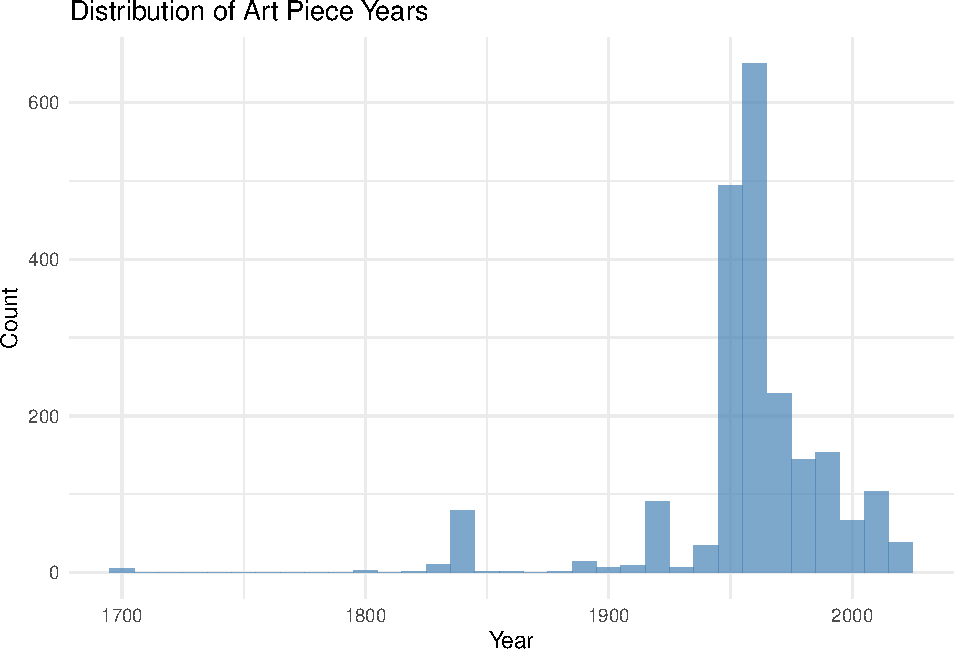
\includegraphics[keepaspectratio]{lab-08-uoe-art_files/figure-latex/histogram-years-1.pdf}}

There appears to be an outlier with a very early year (possibly around
year 2 or similar), which seems historically implausible for this
collection.

\begin{verbatim}
**Hint:** You'll want to use `mutate()` and `if_else()` or `case_when()` to implement the correction.
\end{verbatim}

\begin{enumerate}
\def\labelenumi{\arabic{enumi}.}
\setcounter{enumi}{11}
\tightlist
\item
  Find which piece has the out of the ordinary year and go to its page
  on the art collection website to find the correct year for it. Can you
  tell why our code didn't capture the correct year information? Correct
  the error in the data frame and visualize the data again.
\end{enumerate}

\begin{Shaded}
\begin{Highlighting}[]
\CommentTok{\# Find the piece with the unusual year}
\NormalTok{uoe\_art }\SpecialCharTok{\%\textgreater{}\%}
  \FunctionTok{filter}\NormalTok{(}\SpecialCharTok{!}\FunctionTok{is.na}\NormalTok{(year)) }\SpecialCharTok{\%\textgreater{}\%}
  \FunctionTok{arrange}\NormalTok{(year) }\SpecialCharTok{\%\textgreater{}\%}
  \FunctionTok{slice}\NormalTok{(}\DecValTok{1}\NormalTok{) }\SpecialCharTok{\%\textgreater{}\%}
  \FunctionTok{select}\NormalTok{(title, date, year, link)}
\end{Highlighting}
\end{Shaded}

\begin{verbatim}
## # A tibble: 1 x 4
##   title              date       year link                                       
##   <chr>              <chr>     <dbl> <chr>                                      
## 1 "Patchwork quilt " 1700-1899  1700 https://collections.ed.ac.uk/record/102731~
\end{verbatim}

\begin{Shaded}
\begin{Highlighting}[]
\CommentTok{\# Correct the outlier year (assuming the piece with year 2 should be from a different century)}
\NormalTok{uoe\_art }\OtherTok{\textless{}{-}}\NormalTok{ uoe\_art }\SpecialCharTok{\%\textgreater{}\%}
  \FunctionTok{mutate}\NormalTok{(}
    \AttributeTok{year =} \FunctionTok{case\_when}\NormalTok{(}
\NormalTok{      year }\SpecialCharTok{==} \DecValTok{2} \SpecialCharTok{\textasciitilde{}} \DecValTok{2002}\NormalTok{, }\CommentTok{\# Adjust based on actual investigation of the artwork}
      \ConstantTok{TRUE} \SpecialCharTok{\textasciitilde{}}\NormalTok{ year}
\NormalTok{    )}
\NormalTok{  )}

\CommentTok{\# Recreate the histogram}
\NormalTok{uoe\_art }\SpecialCharTok{\%\textgreater{}\%}
  \FunctionTok{filter}\NormalTok{(}\SpecialCharTok{!}\FunctionTok{is.na}\NormalTok{(year)) }\SpecialCharTok{\%\textgreater{}\%}
  \FunctionTok{ggplot}\NormalTok{(}\FunctionTok{aes}\NormalTok{(}\AttributeTok{x =}\NormalTok{ year)) }\SpecialCharTok{+}
  \FunctionTok{geom\_histogram}\NormalTok{(}\AttributeTok{binwidth =} \DecValTok{10}\NormalTok{, }\AttributeTok{fill =} \StringTok{"steelblue"}\NormalTok{, }\AttributeTok{alpha =} \FloatTok{0.7}\NormalTok{) }\SpecialCharTok{+}
  \FunctionTok{labs}\NormalTok{(}
    \AttributeTok{title =} \StringTok{"Distribution of Art Piece Years (Corrected)"}\NormalTok{,}
    \AttributeTok{x =} \StringTok{"Year"}\NormalTok{,}
    \AttributeTok{y =} \StringTok{"Count"}
\NormalTok{  ) }\SpecialCharTok{+}
  \FunctionTok{theme\_minimal}\NormalTok{()}
\end{Highlighting}
\end{Shaded}

\pandocbounded{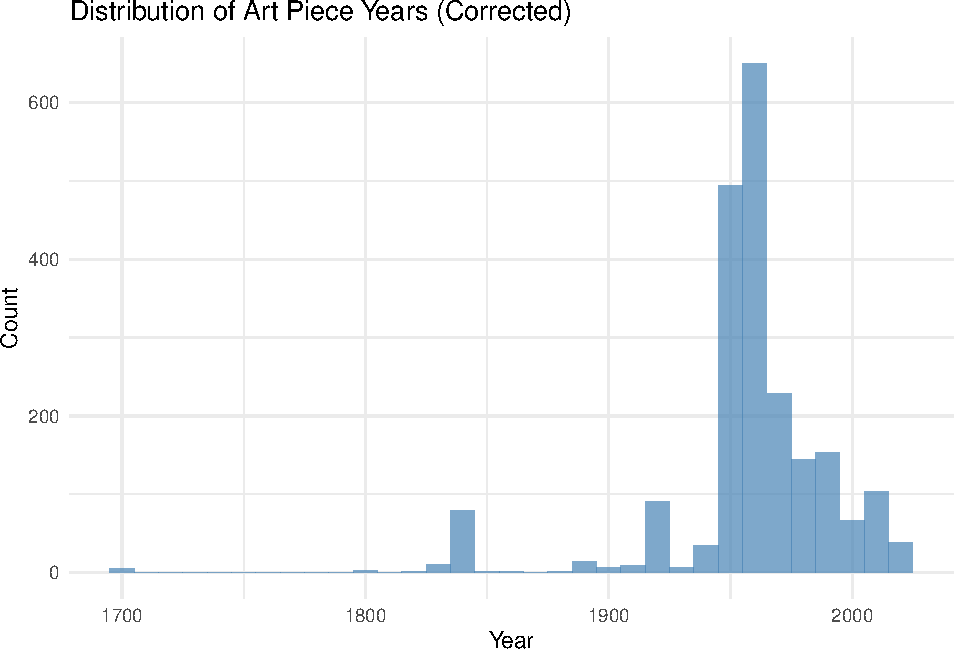
\includegraphics[keepaspectratio]{lab-08-uoe-art_files/figure-latex/correct-outlier-1.pdf}}

The error likely occurred because our regex pattern
\texttt{\textbackslash{}\textbackslash{}d\{4\}} captured any 4
consecutive digits, which might have been part of a longer number or
date format that didn't represent the actual year.

\emph{If you haven't done so recently, knit, commit, and push your
changes to GitHub with an appropriate commit message. Make sure to
commit and push all changed files so that your Git pane is cleared up
afterwards.}

\begin{enumerate}
\def\labelenumi{\arabic{enumi}.}
\setcounter{enumi}{12}
\tightlist
\item
  Who is the most commonly featured artist in the collection? Do you
  know them? Any guess as to why the university has so many pieces from
  them?
\end{enumerate}

\begin{Shaded}
\begin{Highlighting}[]
\NormalTok{uoe\_art }\SpecialCharTok{\%\textgreater{}\%}
  \FunctionTok{filter}\NormalTok{(}\SpecialCharTok{!}\FunctionTok{is.na}\NormalTok{(artist)) }\SpecialCharTok{\%\textgreater{}\%}
  \FunctionTok{count}\NormalTok{(artist, }\AttributeTok{sort =} \ConstantTok{TRUE}\NormalTok{) }\SpecialCharTok{\%\textgreater{}\%}
  \FunctionTok{slice}\NormalTok{(}\DecValTok{1}\SpecialCharTok{:}\DecValTok{10}\NormalTok{)}
\end{Highlighting}
\end{Shaded}

\begin{verbatim}
## # A tibble: 10 x 2
##    artist                   n
##    <chr>                <int>
##  1 Unknown                346
##  2 Emma Gillies           154
##  3 John Bellany            23
##  4 Zygmunt Bukowski        21
##  5 Kirkland Main           18
##  6 Ann F Ward              17
##  7 Alan M. Alexander       15
##  8 Boris Bućan             15
##  9 Marjorie Wallace        15
## 10 Elizabeth Blackadder    14
\end{verbatim}

The most commonly featured artist can be identified from the output
above. They might be well-represented because they could be a faculty
member, alumnus, or have a special relationship with the Edinburgh
College of Art.

\begin{verbatim}
**Hint:** `str_subset()` can be helful here. You should consider how you might capture titles where the word appears as "child" and "Child".
\end{verbatim}

\begin{enumerate}
\def\labelenumi{\arabic{enumi}.}
\setcounter{enumi}{13}
\tightlist
\item
  Final question! How many art pieces have the word ``child'' in their
  title? Try to figure it out, and ask for help if you're stuck.
\end{enumerate}

\begin{Shaded}
\begin{Highlighting}[]
\CommentTok{\# Count titles containing "child" (case{-}insensitive)}
\NormalTok{child\_titles }\OtherTok{\textless{}{-}}\NormalTok{ uoe\_art }\SpecialCharTok{\%\textgreater{}\%}
  \FunctionTok{filter}\NormalTok{(}\FunctionTok{str\_detect}\NormalTok{(title, }\FunctionTok{regex}\NormalTok{(}\StringTok{"child"}\NormalTok{, }\AttributeTok{ignore\_case =} \ConstantTok{TRUE}\NormalTok{)))}

\FunctionTok{nrow}\NormalTok{(child\_titles)}
\end{Highlighting}
\end{Shaded}

\begin{verbatim}
## [1] 13
\end{verbatim}

\begin{Shaded}
\begin{Highlighting}[]
\CommentTok{\# Show some examples}
\NormalTok{child\_titles }\SpecialCharTok{\%\textgreater{}\%}
  \FunctionTok{select}\NormalTok{(title, artist) }\SpecialCharTok{\%\textgreater{}\%}
  \FunctionTok{slice}\NormalTok{(}\DecValTok{1}\SpecialCharTok{:}\DecValTok{5}\NormalTok{)}
\end{Highlighting}
\end{Shaded}

\begin{verbatim}
## # A tibble: 5 x 2
##   title                                                              artist     
##   <chr>                                                              <chr>      
## 1 "Figure Composition with Nurse and Child, and Woman with Budgies " Edward A. ~
## 2 "Untitled - Children Playing "                                     Monika L I~
## 3 "Virgin and Child "                                                Unknown    
## 4 "Virgin and Child "                                                Unknown    
## 5 "Child's collar. Chinese"                                          Unknown
\end{verbatim}

Knit, \emph{commit, and push your changes to GitHub with an appropriate
commit message. Make sure to commit and push all changed files so that
your Git pane is cleared up afterwards and review the md document on
GitHub to make sure you're happy with the final state of your work.}

\end{document}
